\chapter{Réponses aux questions théoriques}\label{chap:Rep}


\section{Modélisation du réseau de Petri}
Nous avons, grâce à \emph{Roméo}, modélisé le système à étudier en un réseau de \textsc{Petri}. Nous avons choisi de représenter le système avec deux files, dont celle allant de l'automate $A$ vers $B$ étant de taille trois et celle allant de $B$ vers $A$ étant de taille deux.

Une fois le système modélisé, l'étude du graphe de marquages (\emph{c.f.} Figure \ref{fig:marquages}) généré par \emph{Roméo} nous apprend qu'il y a toujours au moins un emplacement de chacune des files qui est vide. On peut donc en conclure que pour notre modèle la file de $A$ vers $B$ est bornée à deux ; tandis que le file de $B$ vers $A$ est bornée à un.



\section{Graphe de marquages}
Pour voir la représentation graphique du graphe de marquages, reportez vous à la figure \ref{fig:marquages}.
 \begin{figure}[htb]
   \centering
   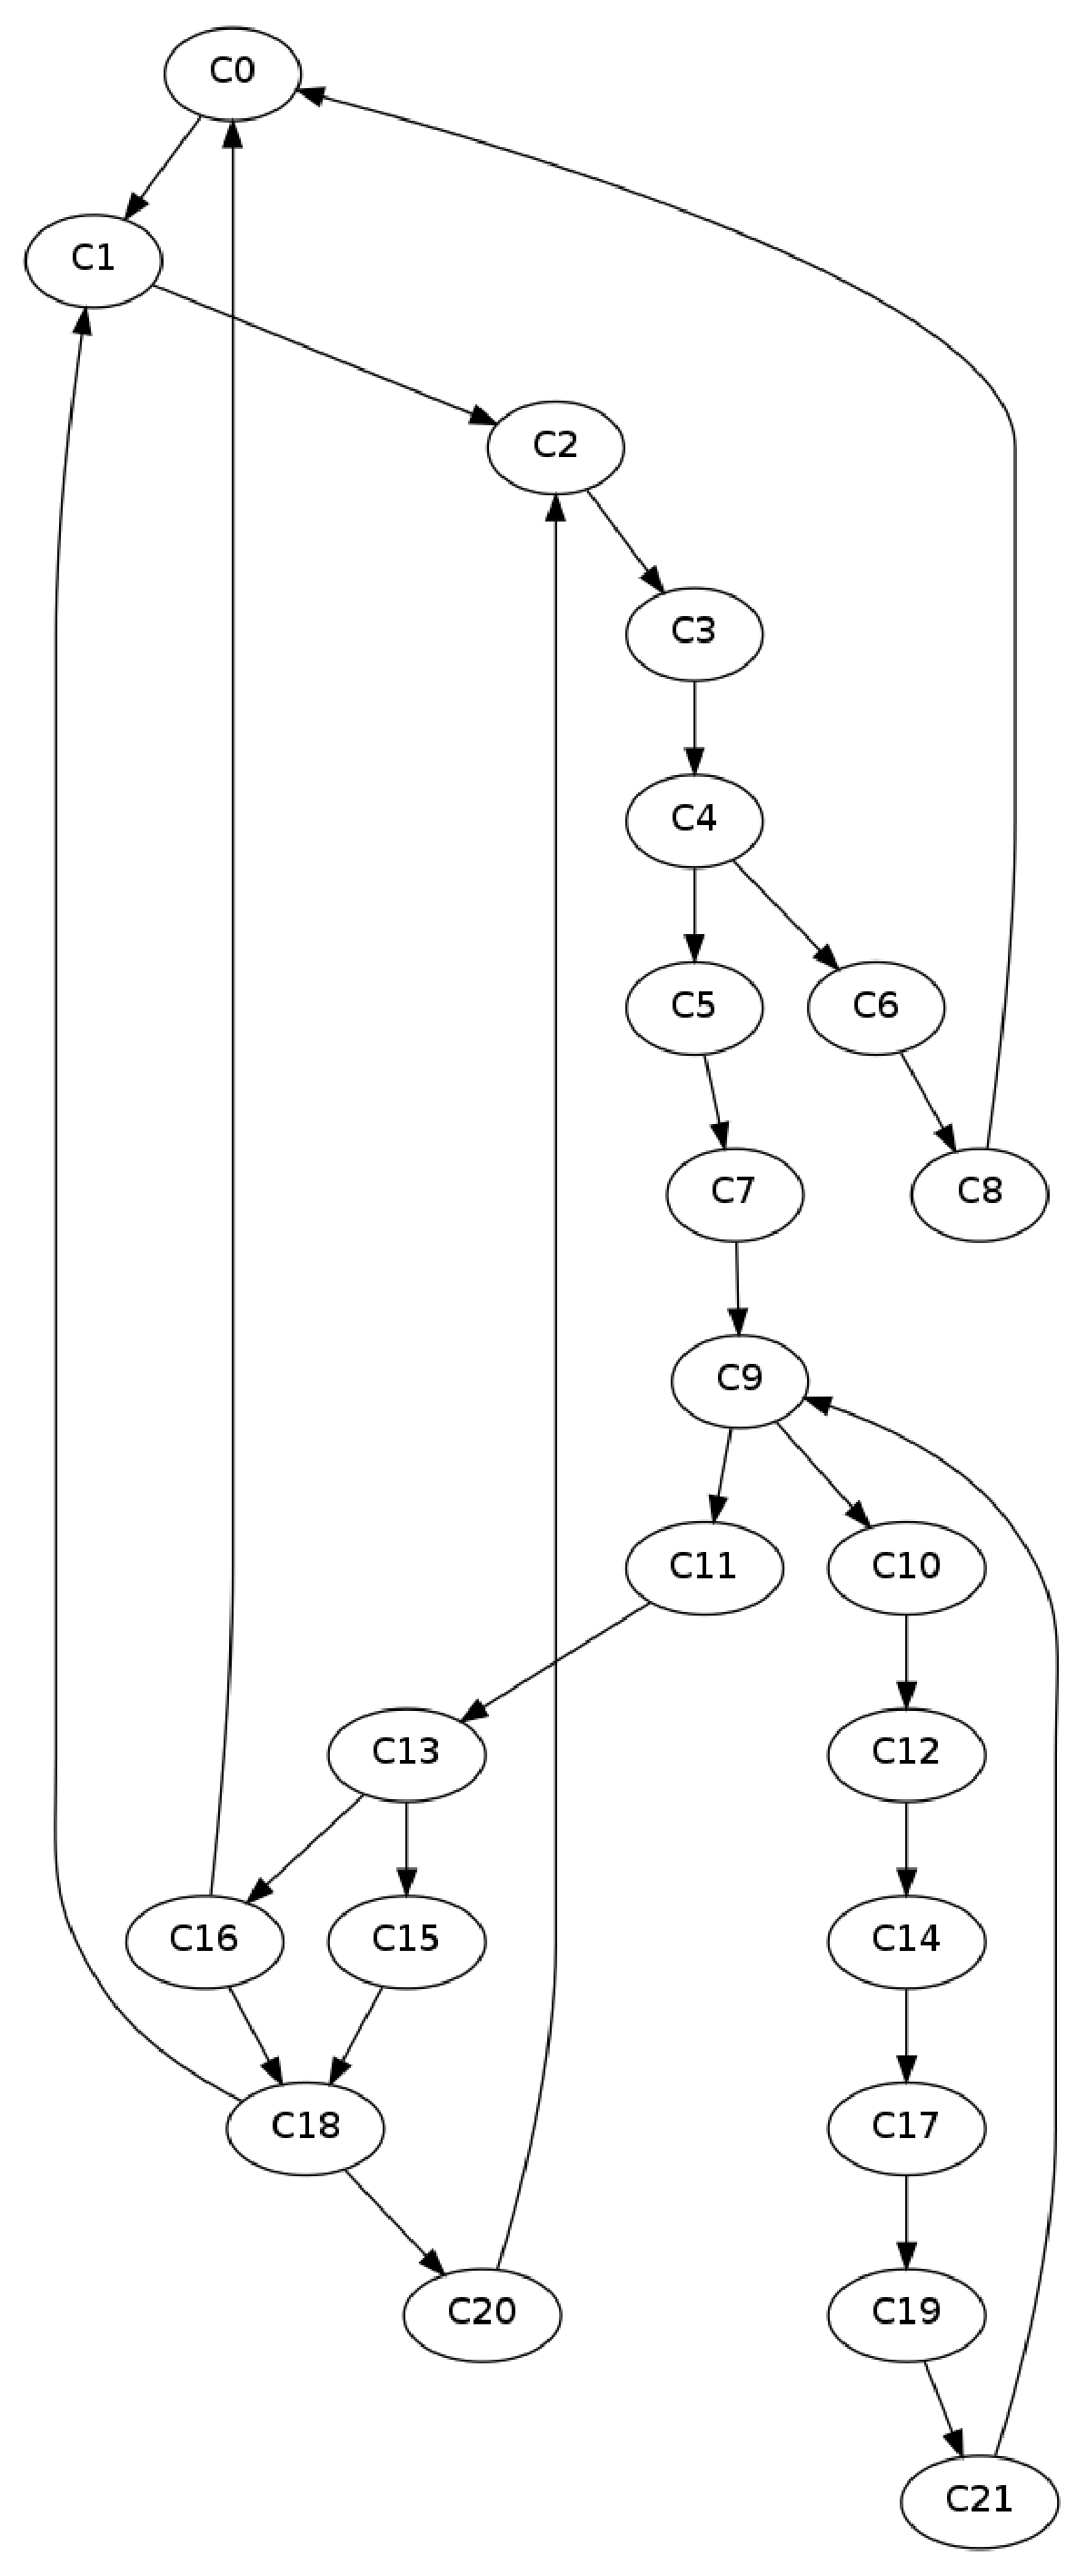
\includegraphics[scale = .3]{img/petri.eps}
   \caption{Graphe des marquages}
   \label{fig:marquages}
 \end{figure}

 
 
 
\section{Logique temporelle}

Deux propositions nous étaient données afin d'être exprimées en logique temporelle:
\begin{enumerate}
 \item Le protocole peut toujours revenir à l’état initial.
 \item Entre deux états où les processus A et B sont en attente, il existe un état où A est déconnecté.
\end{enumerate}
\
Munissons nous de $i$, $i$ faisant partie de notre alphabet pour la logique temporelle et décrivant l'état où A et B sont dans l'état initial. On peut alors exprimer la première proposition de la façon suivante :
\begin{equation}
 \Box\Diamond i
\end{equation}
Pour la seconde proposition, munissons nous de $a$ et $d_A$ appartenant à l'alphabet. $a$ étant l'état où A et B sont en attente et $d_A$ tout état du système où A est déconnecté (dans l'état initial). On peut alors exprimer la seconde proposition de la façon suivante :
\begin{equation}
 \Box((a\wedge\bigcirc\Diamond a)\Longrightarrow(\neg(\neg d_A\cup a)))
\end{equation}
On peut cependant donner une variante où la partie droite de l'implication est modifiée :
\begin{equation}
 \Box((a\wedge\bigcirc\Diamond a)\Longrightarrow\bigcirc(\neg a\cup d_A))
\end{equation}




\section{Étude de la véracité des propositions pour le modèle étudié}
Nous allons à présent déterminer si les deux propositions s'appliquent à notre système. Vous pouvez obtenir une représentation graphique de l'automate du \emph{client} et du \emph{serveur} respectivement sur les figures \ref{fig:ihmCLIENT} et \ref{fig:ihmIA}.

La première proposition est malheureusement ambiguë. En effet il est possible de donner deux sens au verbe \og pouvoir\fg . Si l'on étudie le système on voit qu'il est toujours possible de trouver une suite d'opérations permettant de revenir à l'état initial. Cependant il est aussi possible d'obtenir une suite d'opérations qui ne revient jamais à l'état initial (Notamment lors d'un cas de boucle. \emph{e.g. :} Dans le cas de notre système, on peut opérer un échange de données à l'infini).
Le seconde interprétation de la proposition semble cependant plus en adéquation avec une approche concrète, et donne de plus un contre-exemple. Le système \emph{pourrait} revenir à l'état initial mais cela ne se produira jamais. La première proposition ne semble donc pas valide pour le système étudié.

La seconde proposition est quant à elle plus simple à étudier. Toutes les actions permettant de quitter l'état d'attente (\emph{bgrej} et \emph{bgack}) entraîneront l'automate $A$ soit directement dans l'état déconnecté soit dans un état dans lequel il est nécessaire de passer par la déconnexion de $A$ pour retourner dans l'état d'attente.  La seconde proposition est donc valide pour le système étudié.





% LocalWords:  Roméo Petri c.f e.g bgrej bgack
